\begin{frame}{Biomas}
    \begin{itemize} \setlength\itemsep{1em}
        \item Biomas são:
        \begin{itemize}
            \item Relevo
            \item Cor
        \end{itemize}
        \item Foram implementados cinco biomas distintos
        \item Cada um deles com sues parâmetros para uma função de ruído de Perlin
        \begin{itemize}
            \item $\theta$ quantidade de oitavas
            \item $f$ frequência
        \end{itemize}
        \item Biomas usam maneiras diferente de usar o resultado
        do ruído de Perlin para calcular altura
    \end{itemize}
    
%    \begin{figure}
%        \centering
%        \begin{subfigure}[b]{0.47\textwidth}
%            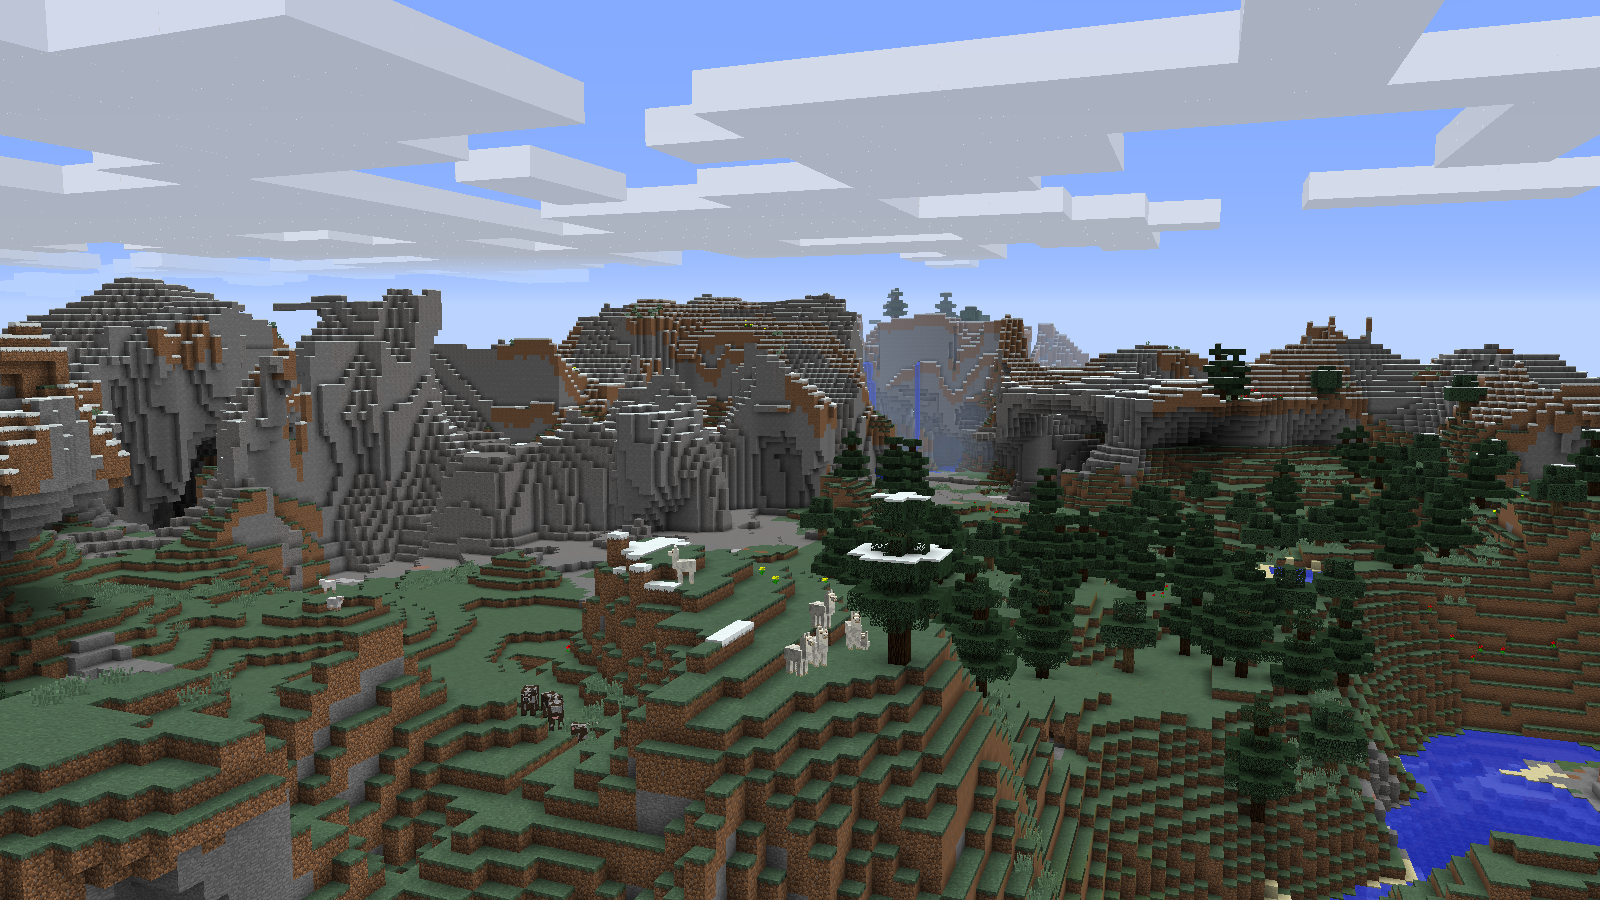
\includegraphics[width=\textwidth]{img/mineExtremeHills}
%            \caption{Bioma \textit{Extreme Hills} no minecraft}
%            \label{fig:mineExtremeHills}
%        \end{subfigure}
%        ~ %add desired spacing between images, e. g. ~, \quad, \qquad, \hfill etc. 
%          %(or a blank line to force the subfigure onto a new line)
%        \begin{subfigure}[b]{0.47\textwidth}
%            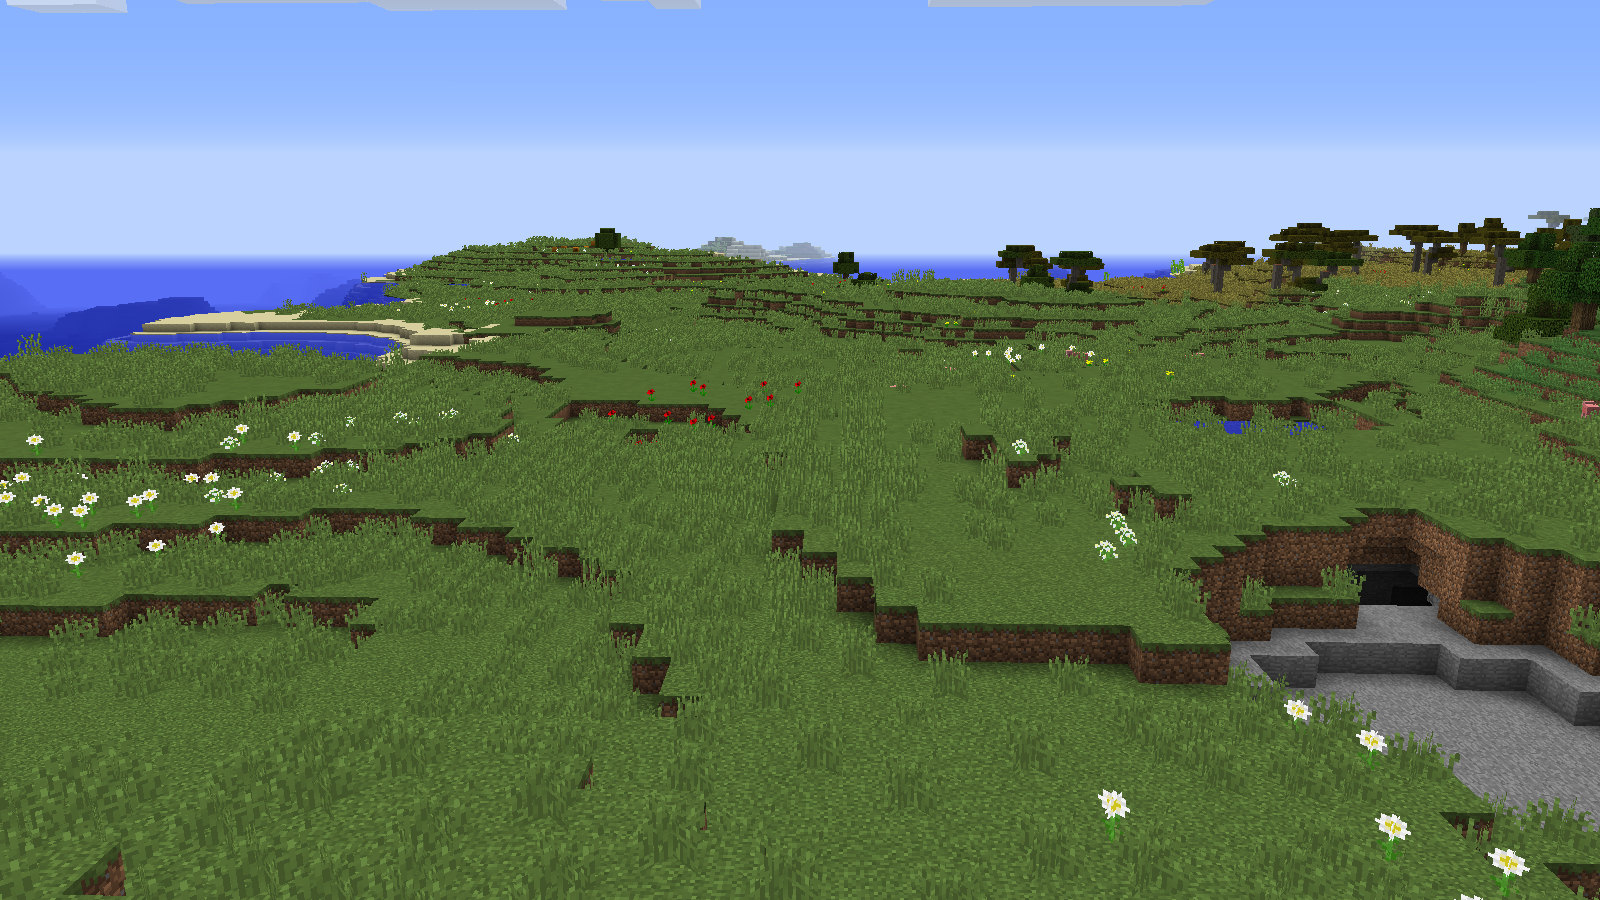
\includegraphics[width=\textwidth]{img/minePlains}
%            \caption{Bioma \textit{Plains} no minecraft}
%            \label{fig:minePlains}
%        \end{subfigure}
%        ~ %add desired spacing between images, e. g. ~, \quad, \qquad, \hfill etc. 
%        %(or a blank line to force the subfigure onto a new line)
%        \caption{Exemplo de Biomas no minecraft}
%        \label{fig:mineBiomes}
%    \end{figure}
    
    
\end{frame}

\begin{frame}{Biomas}
    \begin{figure}[H]
        \centering
        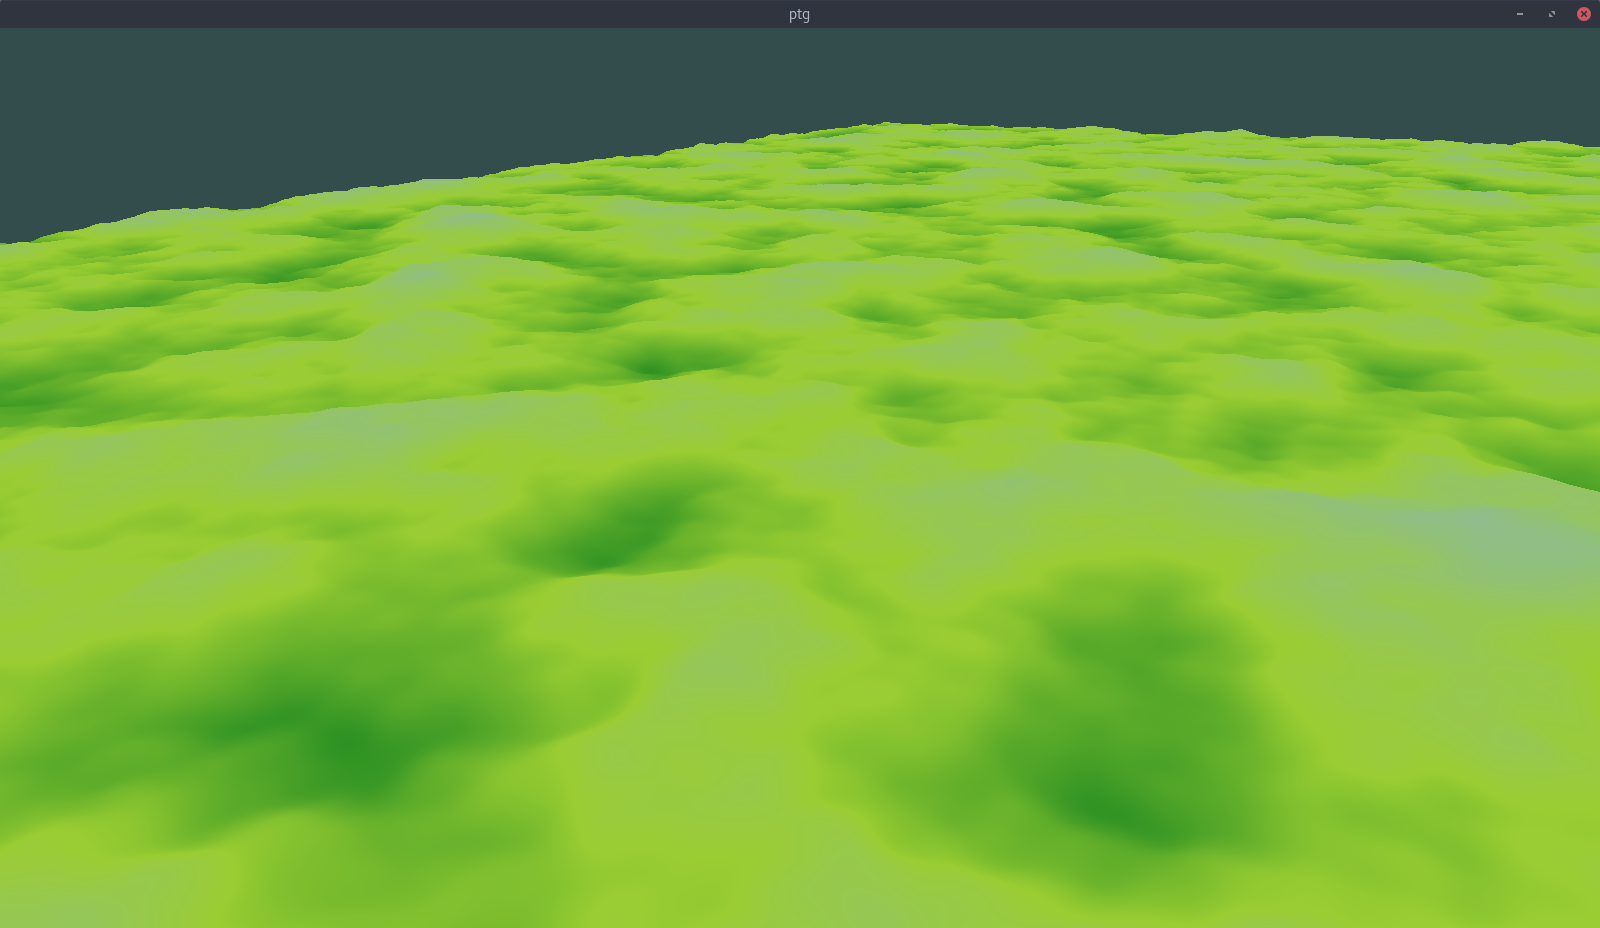
\includegraphics[width=.9\textwidth]{img/biomas/bssPlains.png}
        \caption{Bioma: Planícies, $\theta = 4, f = 10 $.}
        \label{fig:img_biomas_bssPlains}
    \end{figure}
    
    
\end{frame}

\begin{frame}{Biomas}
    \begin{figure}[H]
        \centering
        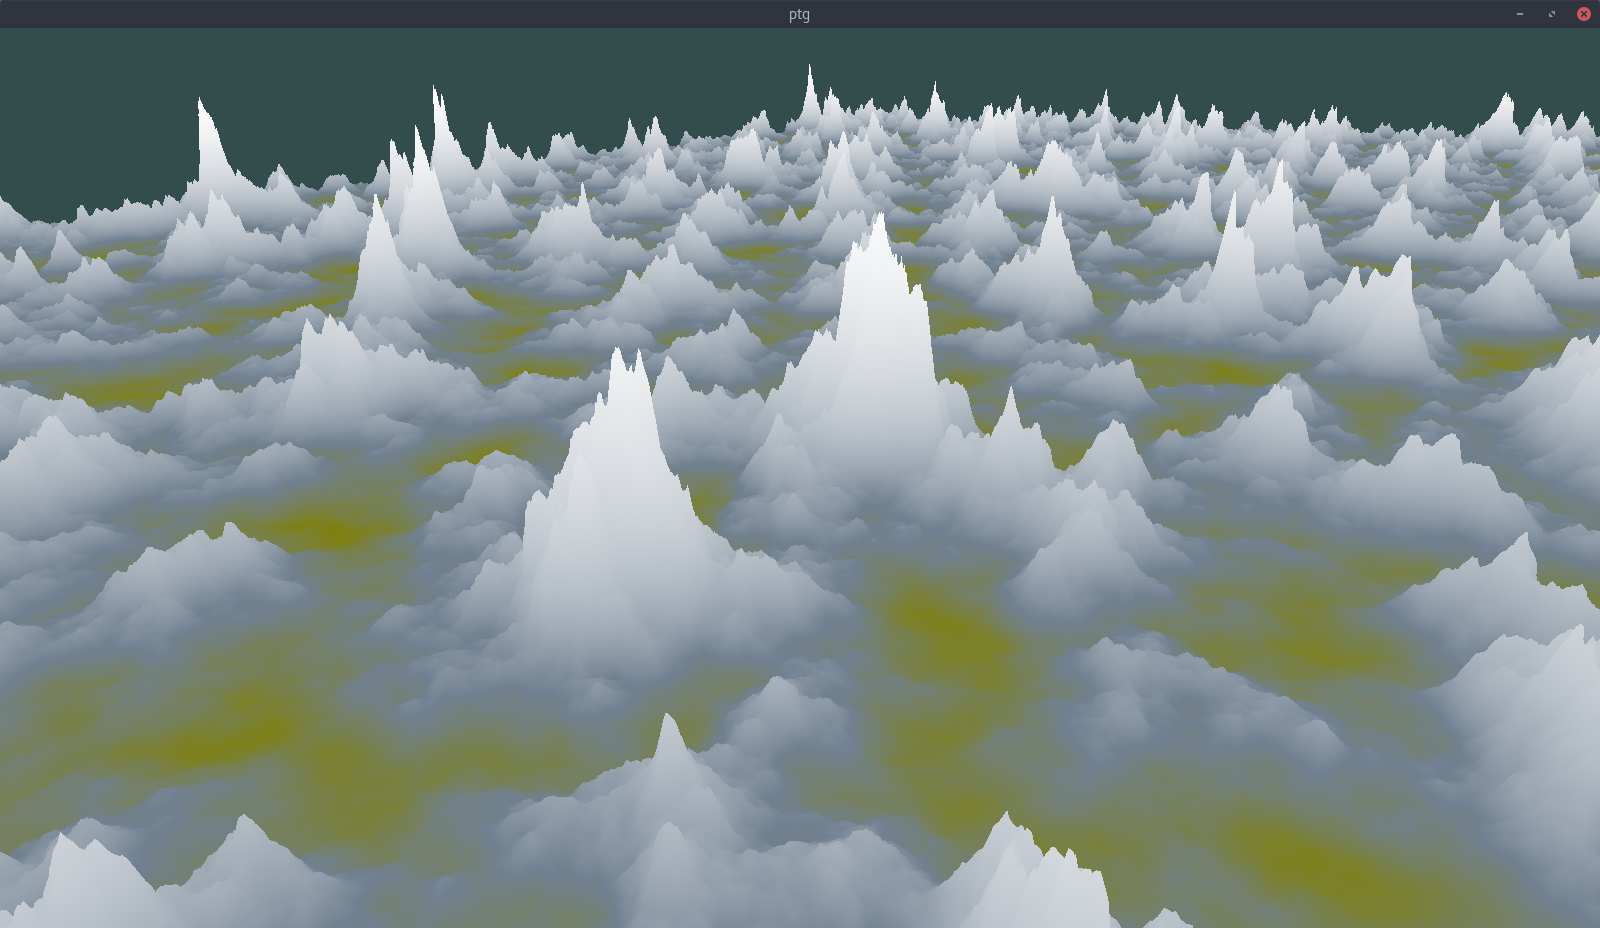
\includegraphics[width=.9\textwidth]{img/biomas/bssMontains.png}
        \caption{Bioma: Montanhas, $\theta =  8, f = 18$.}
        \label{fig:img_biomas_bssMontains}
    \end{figure}
    
    
\end{frame}

\begin{frame}{Biomas}
    \begin{figure}[H]
        \centering
        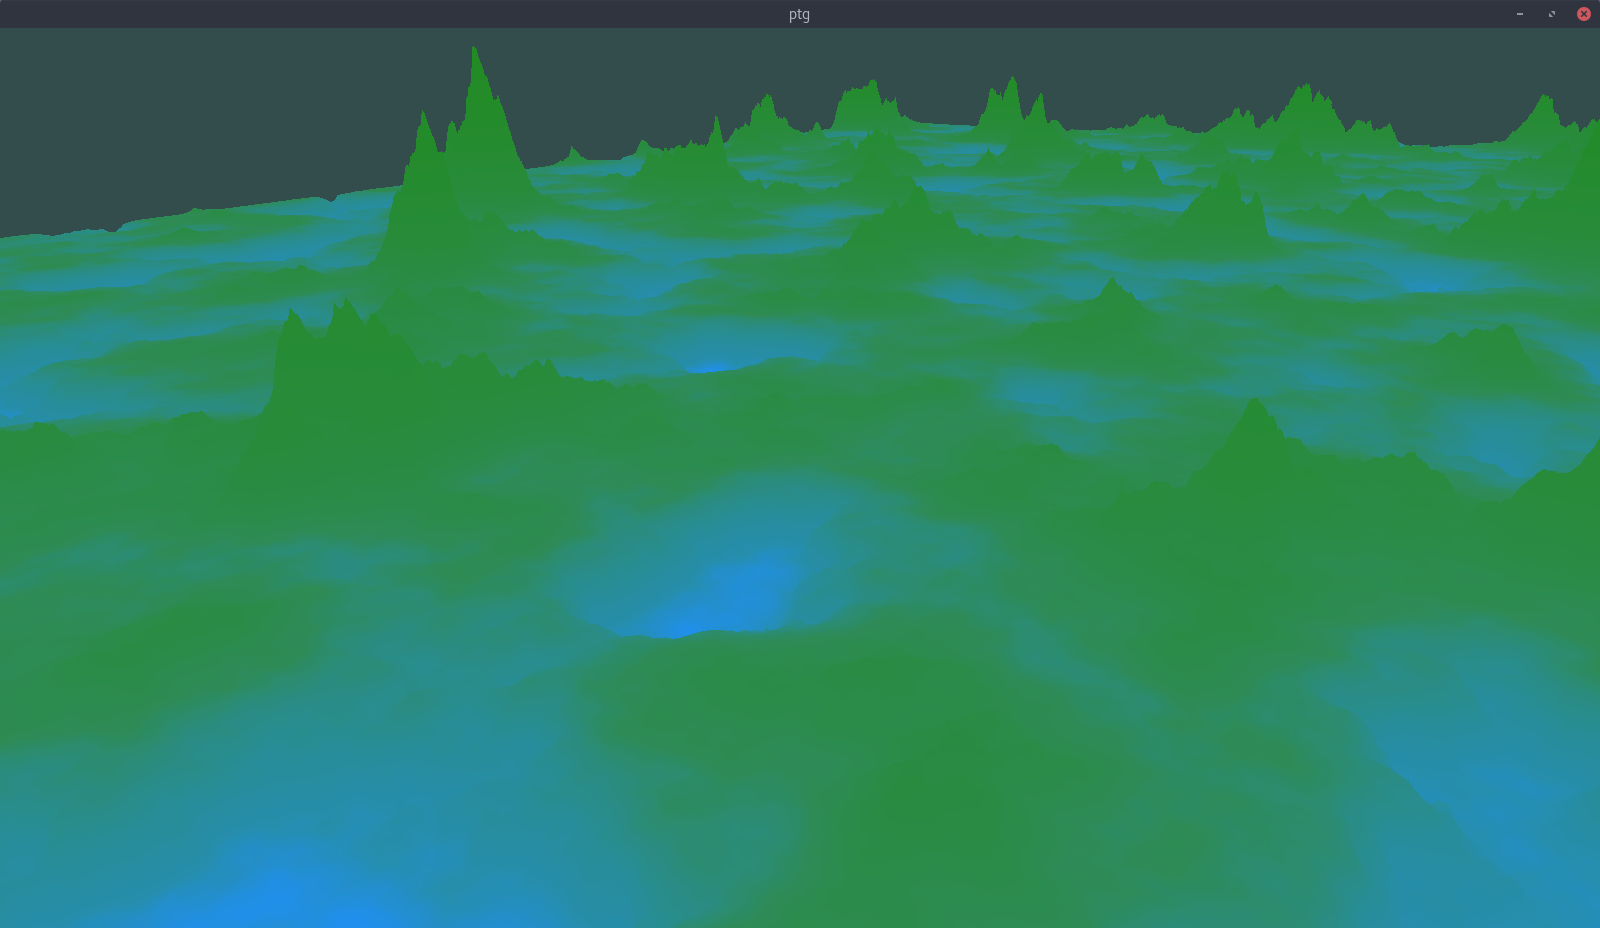
\includegraphics[width=.9\textwidth]{img/biomas/bssValley.png}
        \caption{Bioma: Vales, $\theta = 8, f = 8$.}
        \label{fig:img_biomas_bssValley}
    \end{figure}
    
    
\end{frame}

\begin{frame}{Biomas}
    \begin{figure}[H]
        \centering
        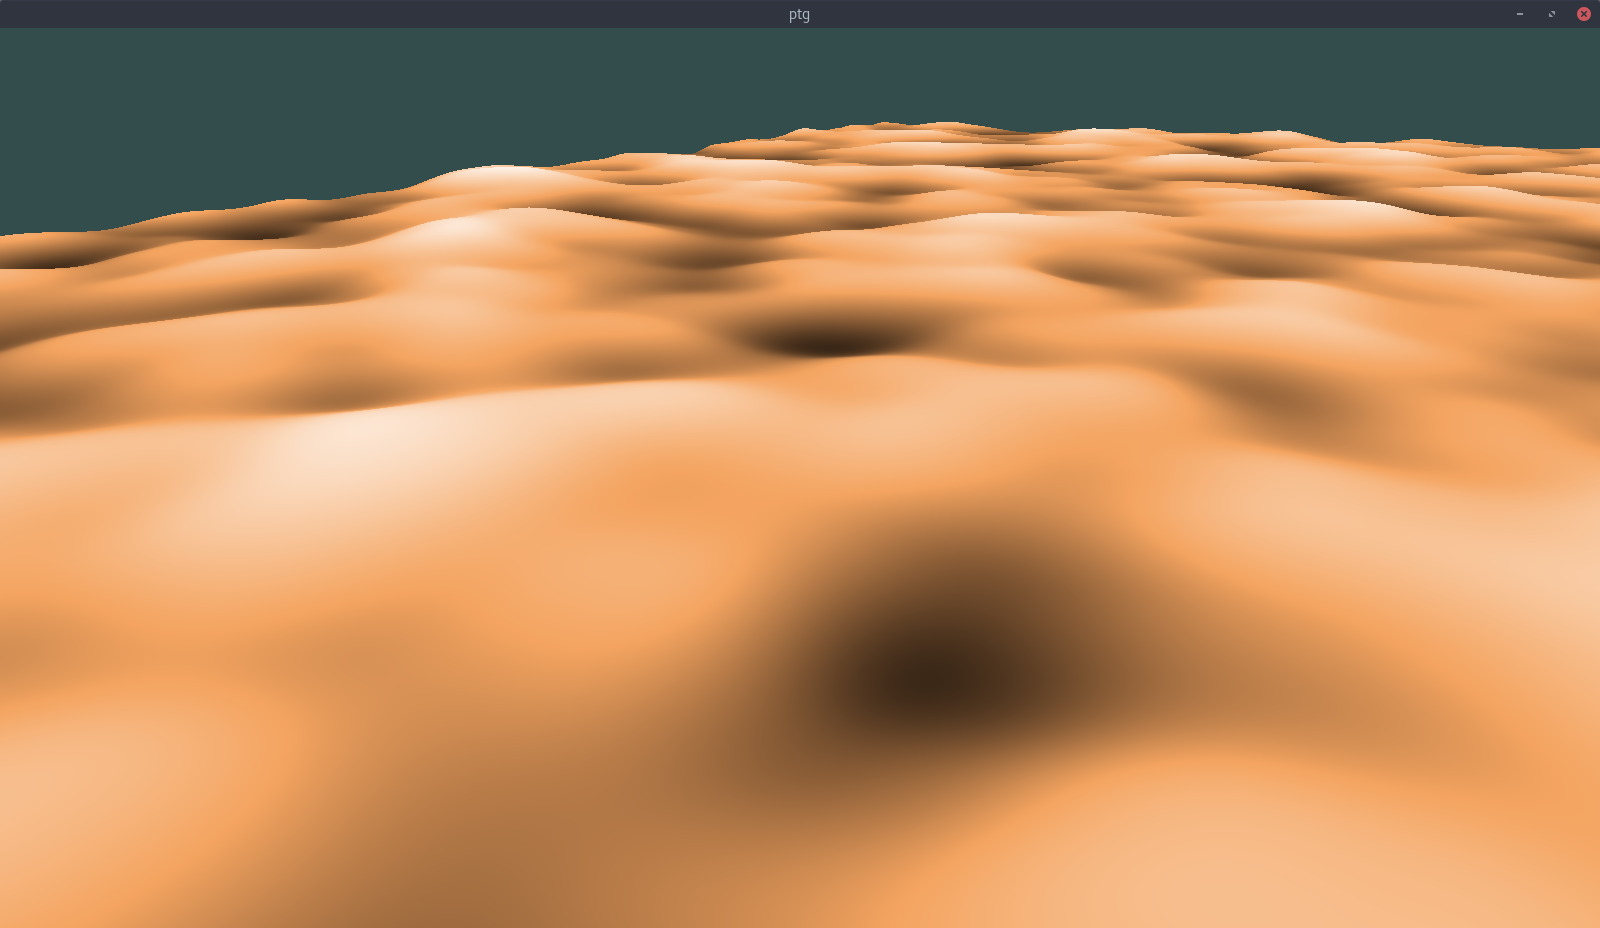
\includegraphics[width=.9\textwidth]{img/biomas/bssDesert.png}
        \caption{Bioma: Deserto, $\theta = 2, f = 6$.}
        \label{fig:img_biomas_bssDesert}
    \end{figure}
    
    
\end{frame}

\begin{frame}{Biomas}
    \begin{figure}[H]
        \centering
        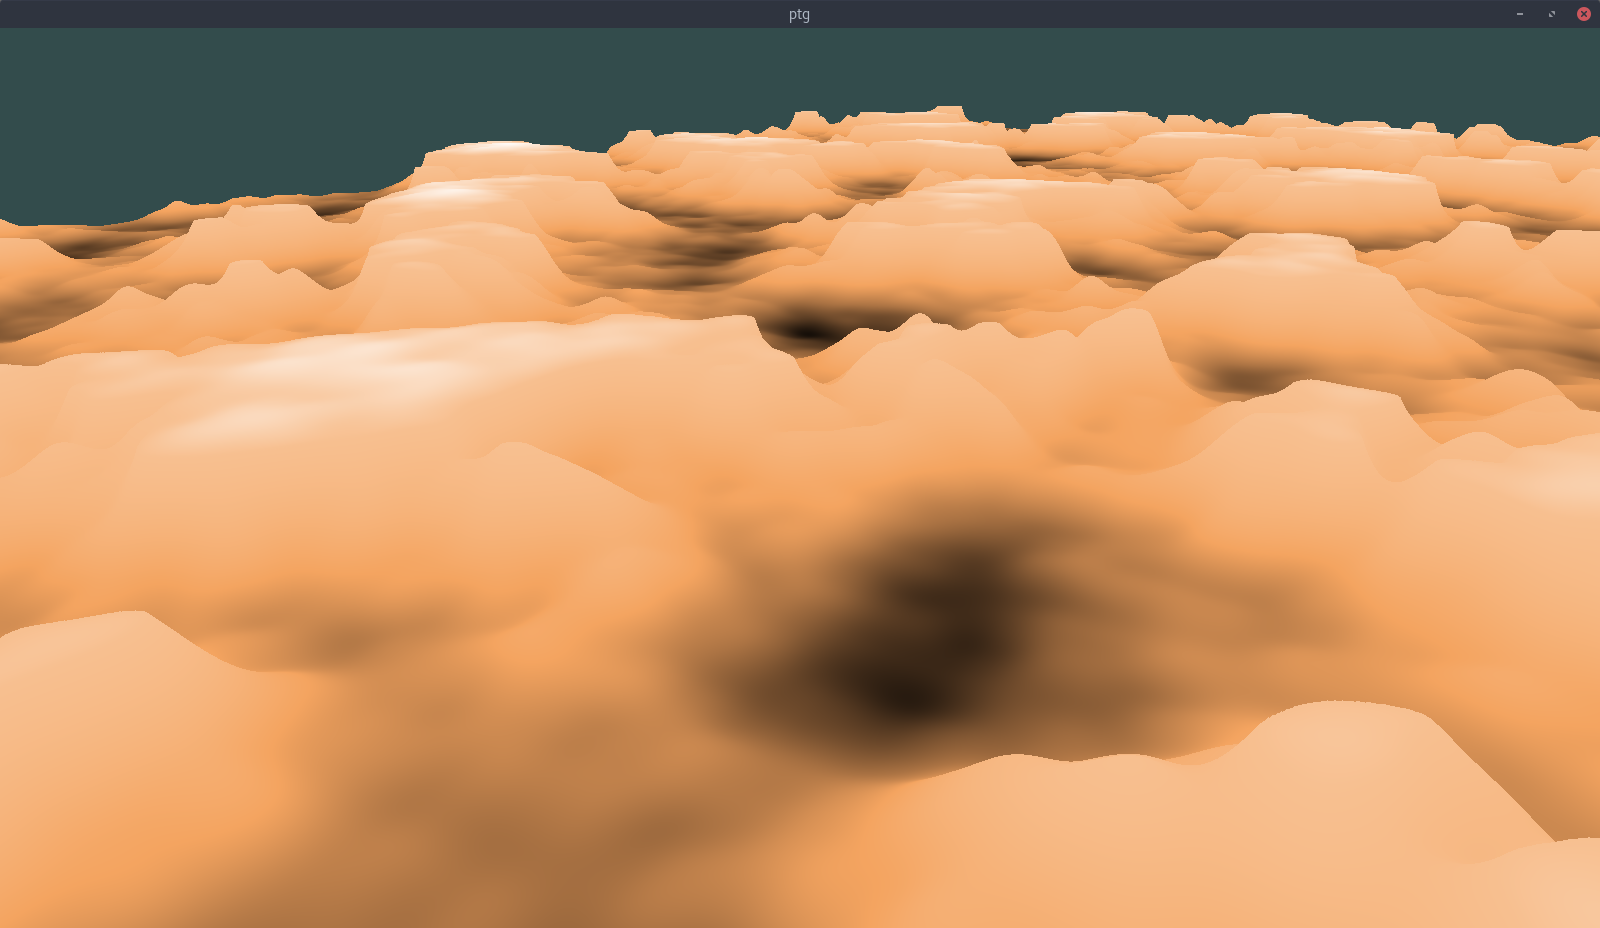
\includegraphics[width=.9\textwidth]{img/biomas/bssCanyons.png}
        \caption{Bioma: Cânyons, $\theta = 4, f = 6$.}
        \label{fig:img_biomas_bssCanyons}
    \end{figure}
    
    
\end{frame}